\chapter{Detección de malware en imágenes}
\label{ch:det_mal}

Durante este capítulo vamos a hablar acerca de la esteganografía, tanto de la tradicional como de la digital; luego pasaremos a revisar la herramienta Stegosploit, necesaria para introducir información oculta en imágenes, junto con el proceso realizado para introducir esa información. Por último veremos FastAI, la solución de inteligencia artificial utilizada para poder detectar malware en imágenes.

\section{¿Qué es la esteganografía?}

La esteganografía es el arte de ocultar información a simple vista dentro, o por encima, de algo que no es secreto (\cite{esteganografia-digital}). Por ejemplo, un documento de texto, un cuadro, una grabación... Sin embargo, esto no es nada nuevo: según la historia, han habido antecedentes que han podido marcar sucesos tan importantes como la Segunda Guerra Mundial, tal y como podemos ver a continuación.%cita

\subsection{Un poco de historia}

Ya en la Antigua Grecia se utilizó para prevenir la invasión del imperio persa: Demarato, antiguo rey de Esparta, tras ser derrocado por Leotíquidas, encontró refugio en la corte del rey de Persia Darío I. Pasó un tiempo e incluso formó parte en la designación de Jerjes como sucesor de Darío. No obstante, a pesar de haber sido expulsado sentía lealtad por su tierra y, cuando los persas se disponían a invadir Grecia, avisó a los griegos mediante mensajes ocultos usando cera para ello; así, pudieron rearmarse y preparar la invasión (\cite{demarato}, \cite{cera-micropuntos}). %cita %cita

Más tarde, en los siglos XVI y XVII también se le daría un buen uso a esta técnica con métodos propuestos a partir de nuevas formas de codificación.

Incluso durante la Primera Guerra Mundial se utilizó tinta invisible como aplicación de esta técnica. Durante la Segunda Guerra Mundial también se llegó a utilizar un método muy interesante: los \textbf{micropuntos}. Los micropuntos, básicamente, eran fotografías del tamaño de una página reducidas hasta ocupar un punto de 1 mm de diámetro y, para ocultarlos, se pegaban sobre un punto del texto que los encubría (\cite{cera-micropuntos}). %cita

\section{Esteganografía digital}

Con la modernización de la sociedad en cuanto a tecnología y computación se refiere, aparecieron diversas aplicaciones de esta técnica con las que se consiguió un nivel de sofisticación y detalle en la técnica adecuado a la época: ahora no sólo era mucho más fácil realizar el escondite del mensaje, también era más complicado detectarlo (\cite{esteganografia-digital}). %cita 

A continuación mencionaremos de forma superficial algunas técnicas de esteganografía digital para poner en contexto la base sobre la que se va a realizar el trabajo:

\subsection{Clasificación tradicional}
\label{sec:trad}

Este tipo de clasificación se basa en cómo se ocultan los datos. A continuación vamos a ver algunas de las técnicas que se comprenden dentro de esta rama:

\subsubsection{Técnicas basadas en la inserción (Insertion-Based)}

Estas técnicas trabajan con la inserción de bloques de datos dentro de un archivo publicable. El dato es insertado en el mismo punto del archivo. Se suelen ocultar en las partes redundantes de un archivo, de forma que el bloque de datos puede estar dividido en varias secciones, haciendo su detección muy difícil (\cite{esteganografia-digital}).%cita

Un ejemplo de uso muy bueno para esta técnica es insertar en los \ac{LSB} de un archivo de 8 ó 16 bits. Lo que se hace es codificar el mensaje en binario e introducirlo dentro de los bits 0, 1, 2 y, tal vez, 3. De esta forma, al ser una de las partes más redundantes de información del archivo, el usuario no es consciente de que ha sido modificado, y por lo tanto puede interactuar con el archivo sin saber que puede haber un mensaje o incluso un malware en su interior que se esté ejecutando.

\subsubsection{Técnicas basadas en algoritmos (Algorithmic-Based)} 

Estas técnicas utilizan alguna clase de algoritmo para decidir dónde se debería ocultar un mensaje dentro de un archivo de datos: es por ello que el bloque de datos no se inserta siempre en el mismo punto, puede estar tanto en las partes más redundantes y olvidadas como en las más importantes... Lo cual es un problema, ya que si no se efectúa bien el algoritmo la ocultación de datos sería fácilmente detectable si se comparan el archivo original con el modificado (\cite{esteganografia-digital}). %cita

El quid de la cuestión de estas técnicas reside en utilizar un algoritmo idóneo para cada tipo de archivo. Optimizando el espacio del archivo con un buen algoritmo, los resultados para la ocultación serán idóneos.

\subsubsection{Técnicas basadas en gramática (Grammar-Based)}

Existe una gran diferencia entre estas técnicas y las anteriores: para las dos primeras se utiliza siempre un archivo que será el que encubra el mensaje... Sin embargo, para estas técnicas se genera un archivo desde cero a partir de los datos a ocultar, basándose en una gramática predefinida (\cite{esteganografia-digital}). %cita

\subsection{Clasificación moderna}

A diferencia de \ref{sec:trad}, esta clasificación se basa en cómo y dónde se ocultan los datos. Es idónea para representar las técnicas desarrolladas en la esteganografía moderna.

\subsubsection{Técnicas basadas en la inserción (Insertion-Based)}

En esencia, se trata de técnicas cuyo objetivo es ocultar datos insertándolos en un archivo sin afectar a su representación, aunque se aumente su tamaño.

Lo bueno de estas técnicas es que se pueden introducir datos en el archivo sin afectar ni modificar el contenido existente. Lo malo es el incremento de tamaño, lo cual es un claro indicador de que se han introducido datos añadidos al archivo.

\subsubsection{Técnicas basadas en la sustitución (Substitution-Based)}

Estas técnicas se basan en sustituir partes del archivo encubridor por los datos a ocultar. De esta forma el tamaño del archivo no varía y, a priori, podría parecer un archivo normal y corriente.

No obstante, es importante aclarar que la sustitución de datos no puede realizarse en cualquier zona del archivo: se corre el riesgo de que al modificarlo, haya partes que queden inservibles o visualmente defectuosas. La clave es encontrar zonas redundantes del archivo y modificarlas para que no se dé ningún impacto.

Otro factor que hay que tener en cuenta es la cantidad de datos que se pueden ocultar en el archivo hasta que éste finalmente no pueda ejecutarse correctamente. En general es una técnica muy buena siempre y cuando se cumplan estas reglas.

\subsubsection{Técnicas de generación (Generation-Based)}

De la misma forma que hemos visto en las técnicas de \ref{sec:trad}, éstas tienen una principal diferencia que cabe destacar: el archivo (o los datos) a ocultar es utilizado para crear el archivo definitivo.

De esta forma, si se consigue únicamente este archivo no debería haber problemas para que el usuario no detecte el mensaje oculto. Si se consigue el archivo original y se compara con el que tiene los datos ocultos se verá que tiene una composición binaria diferente, y la detección esteganográfica será más complicada de realizar.

\section{Stegosploit}

\begin{figure}[H]
  \centering
  
\includegraphics[width=0.60\linewidth]{Figuras/Deteccion\_malware/Stegosploit.png}
  \label{fig:stegosploit}
  \caption{Stegosploit}
\end{figure}

Hemos visto qué clase de técnicas existen para ocultar información en archivos sin que se detecte. No obstante, dentro de las atribuciones de este trabajo nos centraremos en sólo una de ellas, la de sustitución, que es en la que se basa la herramienta que vamos a utilizar para introducir malware en imágenes y sobre la que pretendemos resolver este problema: \textbf{Stegosploit} (\cite{stegosploit}). %cita

Stegosploit es una herramienta creada por el experto en seguridad Saumil Shah (\cite{saumil-shah}) cuyo objetivo es cifrar exploits ``Drive-By Browser'' en imágenes usando esteganografía. De forma resumida, la herramienta cifra los exploits en imágenes JPG y PNG; tras ello, la imagen resultante se fusiona con un HTML con un decodificador en Javascript formando así un \textbf{políglota}: el políglota parece una imagen normal a simple vista, pero se decodifica y se activa en el navegador de la víctima (\cite{stegosploit}). %cita %cita

Para el caso de nuestro trabajo, lo que pretendemos hacer es introducir código malicioso en un set de imágenes usando Stegosploit, en concreto introduciremos este código:

\begin{figure}[H]
  \centering
  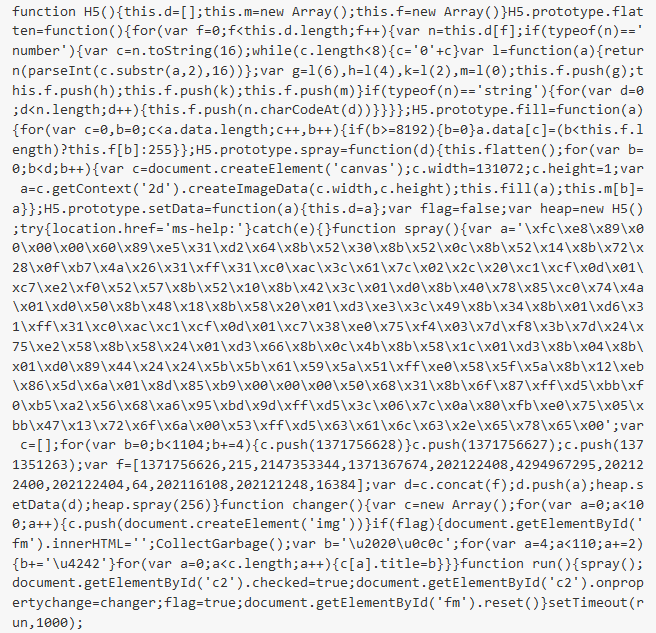
\includegraphics[width=0.60\linewidth]{Figuras/Deteccion\_malware/Stegosploit-2.png}
  \label{fig:exploit}
  \caption{Exploit CVE-2014-0282}
\end{figure}

Antes de empezar, conviene explicar el proceso de encriptado del malware, tal y como viene en la herramienta:

\subsection{Proceso de encriptado}

Para entender el proceso, previamente hay que saber cómo se compone una imagen digital.

Una imagen se compone de píxeles, y cada píxel a su vez se puede componer de tres canales de color: R, G y B (rojo, verde y azul). Cada canal se representa por un valor de 8 bits (es decir 256 colores), de modo que un píxel puede tener hasta 24 bits (\cite{pixel}). %cita

A veces puede haber un cuarto canal llamado ``canal Alpha'', usado para regular la transparencia de los píxeles, es decir, el que se usa para definir la opacidad de un píxel. Sin embargo, en este trabajo no trabajaremos con él, nos centraremos en los tres canales principales (\cite{alpha-channel}). %cita

Una vez explicados los canales, vamos a pasar a representar la imagen como una consecución de capas formadas por los 8 bits de cada canal. Es decir, 8 \textbf{``capas de bit''}. Las capas más externas (la 5, la 6 o la 7) son las más importantes, ya que son las que definen la imagen como tal; es decir, son las que estipulan de qué se compone la imagen y el color principal que ha de aparecer en la misma. Por otro lado, las capas más internas son las más redundantes, ya que a pesar de certificar el color adecuado para cada píxel son capas en las que se puede modificar su valor sin alterar la visualización general de las imágenes. Es justo en las capas más bajas en las que se puede modificar su valor por valores binarios correspondientes al malware a introducir en la imagen. A continuación, veremos en la siguiente figura la estructura de las capas que componen las imágenes:

\begin{figure}[H]
  \centering
  \begin{subfigure}[H]{0.45\linewidth}
  	\includegraphics[width=\linewidth]{Figuras/Deteccion\_malware/Imagen\_Original\_Capas.png}
  	\label{fig:Capas}
  	\caption{Imagen Original}
  \end{subfigure}
  \begin{subfigure}[H]{0.45\linewidth}
  	\includegraphics[width=\linewidth]{Figuras/Deteccion\_malware/Imagen\_Original\_Capas\_1\_0.png}
  	\label{fig:Capas23}
  \caption{Capas 0 y 1}
  \end{subfigure}
  \begin{subfigure}[H]{0.45\linewidth}
  	\includegraphics[width=\linewidth]{Figuras/Deteccion\_malware/Imagen\_Original\_Capas\_3\_2.png}
  	\label{fig:Capas23}
  	\caption{Capas 2 y 3}
  \end{subfigure}
  \begin{subfigure}[H]{0.45\linewidth}
  	\includegraphics[width=\linewidth]{Figuras/Deteccion\_malware/Imagen\_Original\_Capas\_5\_4.png}
  	\label{fig:Capas45}
  \caption{Capas 4 y 5}
  \end{subfigure}
  \begin{subfigure}[H]{0.45\linewidth}
  	\includegraphics[width=\linewidth]{Figuras/Deteccion\_malware/Imagen\_Original\_Capas\_7\_6.png}
  	\label{fig:Capas67}
  \caption{Capas 6 y 7}
  \end{subfigure}
  \caption{Capas de bit de una imagen}
\end{figure}

Como se puede apreciar, y como ya veníamos advirtiendo, las últimas capas son casi ininteligibles para que un ser humano pueda saber de qué trata la imagen; sabiendo esto podemos deducir que son idóneas para la inserción del código malicioso.

Sin embargo, es necesario hacer un apunte muy importante: para nuestro trabajo usaremos un set de imágenes de \textbf{COCO} con formato \textbf{JPG} (\cite{coco}). El formato es muy importante ya que JPG y PNG son dos algoritmos de compresión de imágenes diferentes, y por lo tanto manejan la información de la imagen de diferente manera. %cita

Pasamos a explicar el encriptado en las imágenes \textbf{JPG}, las que tengan un formato \textbf{PNG} las podemos obviar ya que no las usaremos.

\subsubsection{Encriptado en JPG}

JPG es un algoritmo de compresión de imágenes que produce más pérdidas de información de la imagen que PNG, por lo tanto su tratamiento y la introducción de malware serán diferentes. JPG se basa en el uso de la \ac{DCT}, tal y como decíamos en el capítulo anterior, y es por ello que se pierden píxeles de la imagen durante su compresión (\cite{dct}). %cita

Para poder sobrellevar está pérdida y encriptar dentro de la imagen el código vamos a utilizar una técnica de encriptado iterativa, por la cual cuando se desencripte el código no resulte en ningún error.

Antes de comenzar con su explicación primero debemos de señalar la importancia del tamaño de los bloques de datos que se van a encriptar en cada iteración: 

\begin{itemize}
\item Cada encriptado en JPG ofrece una configuración de calidad variable, de esta forma si se aplica una configuración de calidad muy baja se consigue una mayor compresión pero, sin embargo, si se aplica una configuración muy alta tampoco se asegura que la compresión no tenga pérdidas.
\item Ciertos píxeles serán aproximados a sus vecinos independientemente de ello (es decir, adquirirán el valor de sus vecinos).
\item Para minimizar esta aproximación no se debe encriptar el código del exploit que insertaremos en píxeles consecutivos, usaremos en su lugar una \textbf{``parrilla'' (o bloque) de píxeles}.
\item Con esta ``parrilla'' podemos usar las filas y columnas de la misma para encriptar el flujo de bits del malware.
\item Los valores más adecuados para estos bloques suelen ser de \textbf{3x3} o \textbf{4x4}, ya que son los que mejor rinden para este propósito (además de ser una mejor solución para la encriptación que haciéndolo en píxeles consecutivos).
\end{itemize}

Dicho esto, el encriptado en JPG se consigue de la siguiente manera:

\begin{enumerate}
\item Usando el encriptador en JPG que nos proporciona Stegosploit, el mensaje se encripta en la imagen en una de las capas de bit más bajas; dando como resultado una imagen con un mensaje (código) dentro de ella.
\item Si desencriptamos la imagen señalando la capa de bit en la que debería de estar el mensaje, obtenemos el mensaje encriptado... o al menos parte de él, ya que \textbf{JPG es un algoritmo que brinda pérdidas al comprimir la imagen}. Se ha podido perder información del código durante su encriptado, de modo que si se desencripta podría estar incompleto.
\item Si vemos la diferencia entre el mensaje original y el desencriptado, obtenemos un valor \textbf{Delta} que nos indicará el error entre ambos mensajes... Nuestro objetivo es obtener un error de 0.
\item Si volvemos a encriptar el mensaje original en la imagen encriptada por primera vez, obtendremos una nueva imagen con el mismo mensaje pero partiendo de la base de que la imagen con la que se ha encriptado ya ha sido encriptada previamente, por lo que las pérdidas del mensaje durante su desencriptado serán menores.
\item Si ahora decodificamos el mensaje en esta nueva imagen y realizamos el cálculo del error entre el mensaje original y el mensaje desencriptado en esta segunda iteración, obtendremos un valor menor de Delta, es decir, un valor más cercano a 0.
\item Si seguimos iterando, finalmente desencriptaremos el mensaje en claro en algún punto de este proceso.
\end{enumerate}

La herramienta de encriptado de Stegosploit usa la librería del procesador de JPG construida en el navegador desde el que se abre la misma herramienta. Por lo que para el encriptado en JPG es muy importante saber con qué navegador y con qué versión del mismo se va a desencriptar el mensaje (en nuestro caso usaremos \textbf{Firefox v104.0}.

Todo el encriptado esteganográfico se realiza en el propio navegador usando \textbf{Canvas}. %cita

\subsubsection{Canvas}

Canvas es un elemento HTML que, a grandes rasgos, sirve para dibujar gráficos, hacer animaciones y realizar composiciones de fotos (\cite{canvas}).

Para el caso que nos atañe, Canvas se utiliza para obtener los datos de las imágenes en las que vamos a introducir el exploit, es decir, se usa para hacer una copia de la imagen para así poder modificarla desde ese elemento de forma sencilla.

Gracias a Canvas podemos manipular los datos de las imágenes que usaremos y, además, servirá para desencriptar desde el propio navegador el encriptado (cabe recordar que Canvas es un elemento HTML que, dependiendo del navegador, tendrá unas condiciones especiales dentro de su uso). Si usamos el encriptado de JPG en Firefox, el desencriptado en Internet Explorer no será preciso, y de ello depende en parte el uso de Canvas para ambos exploradores, ya que será diferente.

Conviene destacar que en PNG existe la compatibilidad entre diferentes navegadores, sin embargo, y como ya hemos dicho anteriormente, no usaremos imágenes en dicho formato.

\section{FastAI}

Ya hemos visto cómo encriptar el malware en las imágenes JPG, ahora tenemos que ver cómo detectarlo usando herramientas de Deep Learning que, durante el capítulo \ref{ch:stego}, explicaremos con más detalle.

Para usar estas herramientas nos serviremos de \textbf{FastAI}, una solución sencilla que sirve para entrenar modelos de Deep Learning y evaluarlos para diferentes ámbitos (\cite{fastai}). En nuestro caso lo usaremos como un clasificador de imágenes: se realizará la clasificación entre las imágenes que tienen un exploit dentro y las que no. %cita

\subsection{Clasificación de imágenes}

Para clasificar las imágenes previamente debemos etiquetarlas para que, al entrenar los modelos de Deep Learning, éstos sean capaces de saber qué imágenes tienen un exploit (o malware) y cuáles no.

Las etiquetas se definen junto con el resto del código utilizado para: cargar el set de imágenes, entrenar y evaluar el modelo de Deep Learning que hayamos escogido... En el siguiente capítulo lo analizaremos con más detalle.

Una vez etiquetadas las imágenes debemos entrenar los modelos de Deep Learning para su clasificación. La clasificación de imágenes, a priori, puede parecer una solución un tanto ``básica'' para detectar malware dentro de imágenes, ya que al fin y al cabo estamos dictaminando de forma predeterminada qué imágenes tienen un exploit dentro y cuáles no. Sin embargo, con el suficiente entrenamiento para un set de imágenes muy grande, un modelo de Deep Learning puede ser capaz de detectar a nivel de bit la presencia de un exploit dentro de una imagen.

Dicho de otra forma, un set de imágenes con una amplia variedad de éstas que contenga un gran número de imágenes con exploits en su interior podría ser idóneo para que, ante la presencia de una imagen aleatoria, el modelo de Deep Learning sea capaz de analizar la imagen bit a bit y decidir con precisión si hay un exploit en su interior o no.

Es por ello que se necesita una gran cantidad de entrenamientos para múltiples imágenes, para que poco a poco el modelo vaya aprendiendo y, consecuentemente, tenga la capacidad de detectar con solvencia la presencia de estos códigos.

En el siguiente capítulo, veremos la implementación que hemos usado para poner en práctica la teoría aquí explicada, además de los problemas que han aparecido hasta su resolución.